\chapter{Terminal velocity}\label{sec:terminalVelocity}
The equation of motion (Equation~\ref{eqn:equationOfMotion}) described in Section~\ref{sec:theoryOfMagnetophoresis} was studied in order to validate the assumption $d\textbf{v}_{p}/{dt} = 0$. After splitting the equation of motion in its vector components and taking the total derivative one obtains:
\begin{eqnarray}
 m_{p} \frac{du_{p,x}}{dt} &=& V_{p} \Delta \chi \left( B_{x}(x,z) \frac{\partial B_{x}(x,z)}{\partial x} + B_{z}(x,z)\frac{\partial B_{x}(x,z)}{\partial z}\right)\nonumber \\
 & & - 6\pi\eta r_{p} u_{p,x} \label{eqn:diffEquationVx} \\
 m_{p} \frac{du_{p,z}}{dt} &=& V_{p} \Delta \chi \left( B_{x}(x,z) \frac{\partial B_{z}(x,z)}{\partial x} + B_{z}(x,z)\frac{\partial B_{z}(x,z)}{\partial z}\right)\nonumber \\
 & & - 6\pi\eta r_{p} u_{p,z} \label{eqn:diffEquationVy}
\end{eqnarray}

For the sake of simplicity this analysis is done in 2D. The magnetic flux density of the quadrupole arrangement was extracted from ANSYS Maxwell. The gradient of the flux density was calculated numerically at each point using MATLAB. The two differential equations (Equation~\ref{eqn:diffEquationVx} and Equation~\ref{eqn:diffEquationVy}) have been solved in MATLAB by using the built-in differential equation solver $ode45$. The time interval was chosen to be $3$ $\mu$s and the initial conditions were set to $v_{p,x} = v_{p,z} = 0$. Figure~\ref{fig:respondingTime} shows the solution of Equation~\ref{eqn:diffEquationVx} and Equation~\ref{eqn:diffEquationVy}. The results in Figure~\ref{fig:respondingTime} were calculated in the centre of the quadrupole configuration where $x=0$, $y=0$ and $z=0$. It can be seen that the particles reach their terminal velocity in less than $1.5$ $\mu$s when solved for a magnetic flux density between 45 mT and 80 mT. %Even for weak forces, the responding time of the particles were in the same order of magnitude. 

\begin{figure}[htb]
        \centering
        \begin{subfigure}[b]{0.48\textwidth}
                \includegraphics[width=\textwidth]{img/chapters/appendix/terminalVelVx.png}
                \caption{}
                \label{fig:respondingTimeVx}
        \end{subfigure}
        \hfill
        \begin{subfigure}[b]{0.48\textwidth}
                \includegraphics[width=\textwidth]{img/chapters/appendix/terminalVelVy.png}
                \caption{}
                \label{fig:respondingTimeVy}
        \end{subfigure}
        \caption[Responding time of magnetic microparticles]{Responding time of magnetic microparticles in $x$ and $y$ directions. The differential equation is solved for a magnetic $\mathbf{B}$ field of $45$ mT to $80$ mT.}
        \label{fig:respondingTime}
\end{figure}

The responding time of the particle is of the order of $10^{3}$ smaller than time step size used in the simulation. Hence, the assumption made in Equation~\ref{eqn:equationOfMotionSimplified} is valid.

\cleardoublepage

\chapter{Galerkin method}\label{sec:galerkinMethod}
Galerkin method seeks the solution by weighting the residual of the differential equation (Equation~\ref{eqn:vectorPotentialPoissonEquation})~\cite{Jin2014}. By integrating and multiplying both sides of Equation~\ref{eqn:vectorPotentialPoissonEquation} by an arbitrary shape function $w(x)$, the residual can be expressed as:

\begin{equation}
	\int_{X}w(x)\left(\frac{\partial^{2} \Phi(x)}{\partial x^{2}} - f\right)dx = 0
	\label{eqn:weightedResidualsGalerkingMethod}
\end{equation}

The shape function $w(x)$ satisfies the following boundary condition:

\begin{equation}
	w(x) =  0 \text{ on } \partial X
	\label{eqn:shapeFunctionBoundayrCondition}
\end{equation}

Using the boundary condition of $w(x)$ (Equation~\ref{eqn:shapeFunctionBoundayrCondition}) and applying integration by parts, the weak formulation of Equation~\ref{eqn:weightedResidualsGalerkingMethod} can be obtained~\cite{Ciarlet1978,Brenner2008,Oden2012}:

\begin{equation}
	\int_{X} \left( \frac{\partial w(x)}{\partial x}\frac{\partial \Phi(x)}{\partial x} \right) dx + \int_{X} \left( w(x)\Phi(x) \right) dx = 0
	\label{eqn:weakFormulationGalerkinMethod}
\end{equation}

Equation~\ref{eqn:weakFormulationGalerkinMethod} is formulated in a continuous manner. Splitting the domain $X$ into a discrete mesh with elements $e$ one can approximate the continuous function $\Phi(x)$ for each element by $\tilde{\Phi}(x)$, which can be expressed by a linear combination of interpolation functions associated with node values of the finite element mesh:

\begin{equation}
	\Phi(x) \simeq \tilde{\Phi}^{e}(x) = \sum_{i=1}^{m} N_{i}^{e}(x)\hat{\Phi}_{i}^{e} = \{N^{e}\}^{T}\{\hat{\Phi}^{e}\}^{T}
	\label{eqn:functionApproximation}
\end{equation}

where $\hat{\Phi}_{i}^{e}$ is the value of $\Phi$ at node $i$ of element $e$, and $N_{i}^{e}(x)$ is the interpolation function for node $i$. The scalar $m$ is called the degrees of freedom and defines the number of nodes one element has. An important feature of the functions $N_{i}^{e}(x)$ is that they are nonzero only within the element $e$, and outside this element they vanish. Therefore, the nodal shape function $N_{i}^{e}(x)$ can be described by the relation:

\begin{equation*}
N_{i}^{e}(x) = \begin{cases}
1 &\text{at node $i$}\\
0 &\text{at other nodes}
\end{cases}
\end{equation*}

Thus, in 1D the first order interpolation functions in one element $e$ can be expressed as piecewise linear functions:

\begin{eqnarray}
	N_{i}^{e}(x) &= \frac{x_{j}-x}{x_{j}-x_{i}} \\
	N_{j}^{e}(x) &= \frac{x-x_{i}}{x_{j}-x_{i}}
\end{eqnarray}

where $x_{i}$ and $x_{j}$ are the coordinates of the boundaries of one finite elements. The linear interpolation functions are depicted in Figure~\ref{fig:linearShapeFunction}. However, also higher order interpolation functions are possible. One way to build up higher order shape functions is using \emph{Lagrange interpolation functions}, defined by the formula:

\begin{equation}
	N_{i}^{e}(x) = \prod_{j=1, j \neq i}^{m}\frac{x-x_{j}}{x_{i}-x_{j}} 
	\label{eqn:higherOrderInterpolationFunction}
\end{equation}

The second order interpolation function can be defined by three quadratic functions (see Figure~\ref{fig:quadraticShapeFunction}):

\begin{eqnarray}
	N_{i}^{e}(x) &= \frac{(x-x_{j})(x-x_{k})}{(x_{i}-x_{j})(x_{i}-x_{k})}\\
	N_{j}^{e}(x) &= \frac{(x-x_{i})(x-x_{k})}{(x_{j}-x_{i})(x_{j}-x_{k})}\\
	N_{k}^{e}(x) &= \frac{(x-x_{i})(x-x_{j})}{(x_{k}-x_{i})(x_{k}-x_{j})}
\end{eqnarray}

Second order shape functions are able to map gradients more accurately than first order linear functions. The higher order polynomials, although very accurate, usually result in a more complicated formulation. Hence, the simple linear or quadratic interpolation is mostly used~\cite{Jin2014}. 

\begin{figure}[htb]
        \centering
        \begin{subfigure}[b]{0.45\textwidth}
                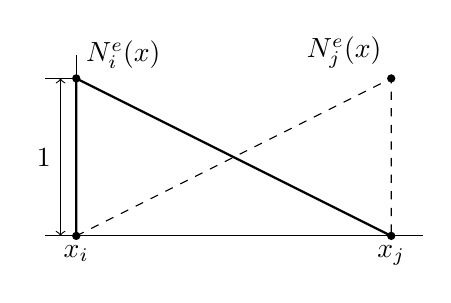
\begin{tikzpicture}[scale=1.0]
                
                \draw (-0.4,0) -- (4.4,0);
                \draw (0,0) -- (0,2.3);
                
				\coordinate[label=below:$x_{i}$] 			(x1) at (0,0);
				\coordinate[label=below:$x_{j}$] 			(x2) at (4,0);
				\coordinate[label=above right:$N_{i}^{e}(x)$] 	(y1) at (0,2);
				\coordinate[label=above left:$N_{j}^{e}(x)$] 	(y2) at (4,2);				
		
				\draw[dashed] (x1) -- (y2) --  (x2);
				\draw[thick] (x1) -- (y1) -- (x2);
	
				\fill (x1) circle (1.5pt);	
				\fill (x2) circle (1.5pt);
				\fill (y1) circle (1.5pt);
				\fill (y2) circle (1.5pt);

				\draw (0,2) -- (-0.4,2);				
				\draw[<->] (-0.2,0) -- node[left]{$1$} (-0.2,2);
				
				\end{tikzpicture}
                \caption{Linear}
                \label{fig:linearShapeFunction}
        \end{subfigure}
        \begin{subfigure}[b]{0.45\textwidth}
                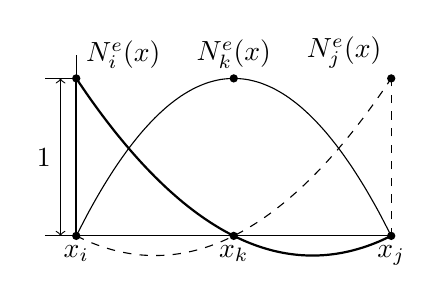
\begin{tikzpicture}[scale=1.0]
                
                \draw (-0.4,0) -- (4,0);
                \draw (0,0) -- (0,2.3);
                
				\coordinate[label=below:$x_{i}$] 				(x1) at (0,0);
				\coordinate[label=below:$x_{j}$] 				(x2) at (4,0);
				\coordinate[label=below:$x_{k}$] 				(x3) at (2,0);
				\coordinate[label=above right:$N_{i}^{e}(x)$] 	(y1) at (0,2);
				\coordinate[label=above left:$N_{j}^{e}(x)$] 	(y2) at (4,2);	
				\coordinate[label=above:$N_{k}^{e}(x)$] 		(y3) at (2,2);				
		
				\draw[thick,domain=0:4,smooth,variable=\x,black] plot ({\x},{2*(\x-4)*(\x-2)/((0-4)*(0-2))});
				\draw[thick] (x1)--(y1);
				\draw[dashed,domain=0:4,smooth,variable=\x,black] plot ({\x},{2*(\x-0)*(\x-2)/((4-0)*(4-2))});
				\draw[dashed] (x2) -- (y2);
				\draw[domain=0:4,smooth,variable=\x,black] plot ({\x},{2*(\x-0)*(\x-4)/((2-0)*(2-4))});
					
				\fill (x1) circle (1.5pt);	
				\fill (x2) circle (1.5pt);
				\fill (x3) circle (1.5pt);
				\fill (y1) circle (1.5pt);
				\fill (y2) circle (1.5pt);
				\fill (y3) circle (1.5pt);
				
				\draw (0,2) -- (-0.4,2);				
				\draw[<->] (-0.2,0) -- node[left]{$1$} (-0.2,2);
				
				\end{tikzpicture}
                \caption{Quadratic}
                \label{fig:quadraticShapeFunction}
        \end{subfigure}
        \caption[Different shape functions in a single element]{1D first (linear) and second (quadratic) order shape functions in a single element $e$ where $x_{i}$ and $x_{j}$ are the two nodes of the linear element.}
        \label{fig:shapeFunction}
\end{figure}

The continuous function $\Phi(x)$ has now been transformed into a set of discrete values $(x_{i},\hat{\Phi}_{i}^{e})$ multiplied by an interpolation function $N_{i}^{e}(x)$. The Galerkin method, replaces the weighting functions $w(x)$ with the interpolation functions $N^{e}(x)$ used for the expansion of the approximate solution. This usually leads to the most accurate solution and is therefore a popular approach~\cite{Jin2014,Ciarlet1978,Brenner2008,Oden2012}. Thus, replacing $\Phi(x)$ by its approximation $\tilde{\Phi}(x)$ in Equation~\ref{eqn:weakFormulationGalerkinMethod} and also select the weighting functions $w(x)$ to be the same as those used for the expansion of the approximation the continuous weak formulation can be written in a discrete form:

\begin{equation}
 	\sum_{e}\biggl\{\int_{x_{i}}^{x_{j}}\left(\frac{\partial \{N^{e}\}^{T}}{\partial x}\frac{\partial N^{e}}{\partial x}\hat{\Phi}^{e}\right)dx - \int_{x_{i}}^{x_{j}}\bigg(\{N^{e}\}^{T}f\bigg)dx \biggl\} = 0
 	\label{eqn:weakFormulationGalerkinMethodDiscrete}
\end{equation}

where $e$ is the element between two consecutive points $x_{i}$ and $x_{j}$. Equation~\ref{eqn:weakFormulationGalerkinMethodDiscrete} can also be written in matrix notation:

\begin{align}
	\mathbf{\Pi}\hat{\Phi} &= \textbf{f} \label{eqn:matrixNotationGalerkinMethod}\\	
	\text{with} \nonumber \\
	\mathbf{\Pi} &= \sum_{e} \biggl\{ \int_{x_{i}}^{x_{j}} \frac{\partial \{N^{e}\}^{T}}{\partial x}\frac{\partial N^{e}}{\partial x} \biggl\} \label{eqn:eqn:stiffnessMatrixGalerkinMethod}\\
	\textbf{f} &= \sum_{e} \biggl\{ \int_{x_{i}}^{x_{j}} \{N^{e}\}^{T}f \biggl\} \label{eqn:rightHandSideGalerkinMethod}
\end{align}
	
The matrix $\mathbf{\Pi}$ and vector $\mathbf{f}$ are often referred to as \emph{stiffness matrix} and \emph{load vector}, respectively, names originally coming from the context of structural problems~\cite{Ciarlet1978,Jin2014}. 

Equation~\ref{eqn:matrixNotationGalerkinMethod} can easily be computed using MATLAB. A possible solution is shown in Figure~\ref{fig:possibleFemSolution}. 

\begin{figure}[htb]
\centering
\begin{tikzpicture}[scale=0.9]
	\coordinate[label=below:$x_{0}$] 	(A) at (0,0);
	\coordinate[label=below:$x_{1}$] 	(B) at (4,0);
	\coordinate[label=below:$x_{2}$] 	(C) at (8,0);
	\coordinate[label=below:$x_{3}$] 	(D) at (12,0);
	
	\coordinate[label=above:$\hat{\Phi}_{0}$] 	(E) at (0,4);
	\coordinate[label=above:$\hat{\Phi}_{1}$] 		(F) at (4,3);
	\coordinate[label=above:$\hat{\Phi}_{2}$] 	(G) at (8,1);
	\coordinate[label=above:$\hat{\Phi}_{3}$] 	(H) at (12,4);
	
	\draw (A) -- (B) -- (C) -- (D);
	\draw (A) -- (E);
	\draw (B) -- (F);
	\draw (C) -- (G);
	\draw (D) -- (H);
	\draw (E) -- (F) -- (G) -- (H);
	\fill (A) circle (1.5pt);
	\fill (B) circle (1.5pt);
	\fill (C) circle (1.5pt);
	\fill (D) circle (1.5pt);
	\fill (E) circle (1.5pt);
	\fill (F) circle (1.5pt);
	\fill (G) circle (1.5pt);
	\fill (H) circle (1.5pt);
\end{tikzpicture}
\caption[FEM solution example]{Possible FEM solution to the initial differential equation problem given in Equation~\ref{eqn:vectorPotentialPoissonEquation}. Values between two nodes are approximated by linear functions.}%
\label{fig:possibleFemSolution}%
\end{figure}

Since the solution of Equation~\ref{eqn:vectorPotentialPoissonEquation} is only approximated by $\tilde{\Phi}(x)$, the residuals calculated in Equation~\ref{eqn:weightedResidualsGalerkingMethod} do not sum to zero. Therefore, substitution of $\tilde{\Phi}(x)$ for $\Phi(x)$ in Equation~\ref{eqn:weightedResidualsGalerkingMethod} would then result in a nonzero residual, where the best approximation minimizes the residual equation:

\begin{equation}
	\int_{X} w(x)\left(\frac{\partial^{2} \tilde{\Phi}(x)}{\partial x^{2}} - f \right) dx \neq 0
	\label{eqn:weightedResidualsGalerkingMethodNoneZero}
\end{equation}

\cleardoublepage

\chapter{Magnetic bead imaging}\label{sec:magneticBeadImaging}
All magnetic bead types have been imaged using scanning electron microscopy (SEM). The SEM images are used to visualize the particles' shape and to estimate their size distribution. The following pictures show the SEM images of the various particle types.

\begin{figure}[htb]
	\centering
    \begin{subfigure}[b]{0.48\textwidth}
		\includegraphics[width = \textwidth]{img/chapters/appendix/screenMag_01_i002.jpg}
        \caption{}
	\end{subfigure}
    \hfill
	\begin{subfigure}[b]{0.48\textwidth}
    	\includegraphics[width = \textwidth]{img/chapters/appendix/screenMag_01_i010.jpg}
    	\caption{}
    \end{subfigure}
	\hfill
	\begin{subfigure}[b]{0.48\textwidth}
		\includegraphics[width = \textwidth]{img/chapters/appendix/screenMag_01_i014.jpg}
		\caption{}
	\end{subfigure}
	\caption[SEM images for Chemicell ScreenMAG particles including measurements]{SEM images of the Chemicell ScreenMAG particles including their diameter measurement.}
\label{fig:}
\end{figure}

\begin{figure}[htb]
	\centering
	\begin{subfigure}[b]{0.48\textwidth}
		\includegraphics[width = \textwidth]{img/chapters/appendix/siMag_01_i001.png}
		\caption{}
	\end{subfigure}
	\hfill
	\begin{subfigure}[b]{0.48\textwidth}
		\includegraphics[width = \textwidth]{img/chapters/appendix/siMag_01_i002.png}
		\caption{}
	\end{subfigure}
	\hfill
	\begin{subfigure}[b]{0.48\textwidth}
		\includegraphics[width = \textwidth]{img/chapters/appendix/siMag_01_i009.png}
		\caption{}
	\end{subfigure}
	\caption[SEM image for Chemicell SiMAG particles including measuremen]{SEM image of the Chemicell SiMAG particles including their diameter measurement.}
\end{figure}

\begin{figure}[htb]
	\centering
	\begin{subfigure}[b]{0.48\textwidth}
		\includegraphics[width = \textwidth]{img/chapters/appendix/myOne_01_i008.png}
		\caption{}
	\end{subfigure}
	\hfill
	\begin{subfigure}[b]{0.48\textwidth}
		\includegraphics[width = \textwidth]{img/chapters/appendix/myOne_01_i022.png}
		\caption{}
	\end{subfigure}
	\hfill
	\begin{subfigure}[b]{0.48\textwidth}
		\includegraphics[width = \textwidth]{img/chapters/appendix/myOne_01_i035.png}
		\caption{}
	\end{subfigure}
	\caption[SEM images for Dynabead MyOne particles including measurements]{SEM images of the Dynabead MyOne particles including their diameter measurement.}
\end{figure}

\begin{figure}[htb]
	\centering
	\begin{subfigure}[b]{0.48\textwidth}
		\includegraphics[width = \textwidth]{img/chapters/appendix/m280_01_i012.png}
		\caption{}
	\end{subfigure}
	\hfill
	\begin{subfigure}[b]{0.48\textwidth}
		\includegraphics[width = \textwidth]{img/chapters/appendix/m280_01_i017.png}
		\caption{}
	\end{subfigure}
	\hfill
	\begin{subfigure}[b]{0.48\textwidth}
		\includegraphics[width = \textwidth]{img/chapters/appendix/m280_01_i023.png}
		\caption{}
	\end{subfigure}
	\caption[SEM images for Dynabead M280 particles including measurements]{SEM images of the Dynabead M280 particles including their diameter measurement.}
\end{figure}

\begin{figure}[htb]
	\centering
	\begin{subfigure}[b]{0.48\textwidth}
		\includegraphics[width = \textwidth]{img/chapters/appendix/m270_04_i023.jpg}
		\caption{}
	\end{subfigure}
	\hfill
	\begin{subfigure}[b]{0.48\textwidth}
		\includegraphics[width = \textwidth]{img/chapters/appendix/m270_04_i029.jpg}
		\caption{}
	\end{subfigure}
	\hfill
	\begin{subfigure}[b]{0.48\textwidth}
		\includegraphics[width = \textwidth]{img/chapters/appendix/m270_04_i033.jpg}
		\caption{}
	\end{subfigure}
	\caption[SEM images for Dynabead M270 particles including measurements]{SEM images of the Dynabead M270 particles including their diameter measurement.}
\end{figure}

\cleardoublepage

\chapter{Finite element method validation}\label{sec:femValidation}
In order to evaluate the solution computed by ANSYS Maxwell a mesh independence study is performed, where the number of nodes in the mesh has been gradually increased until no significant change in the solution can be detected. The study is done using a bar magnet as a canonical example, as shown in Figure~\ref{fig:barMagnetScheme}. The chosen magnet geometry is also used in this thesis and thus conducting a grid independence analysis for this design also has an application value.

\begin{figure}[htb]
\centering
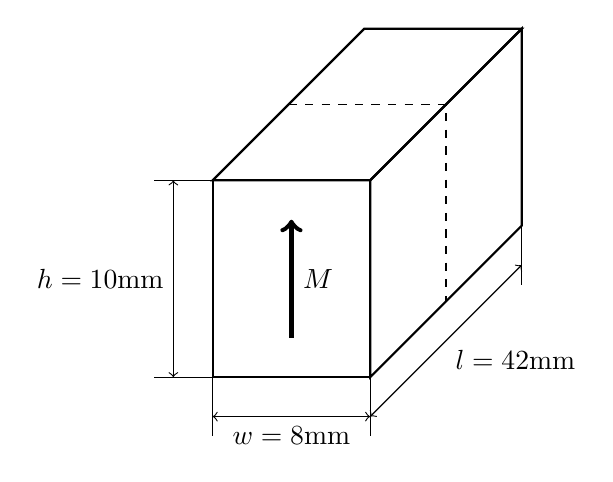
\begin{tikzpicture}[scale=1.0]
	\coordinate 	(A) at (0,0,0);
	\coordinate 	(B) at (2,0,0);
	\coordinate 	(C) at (2,2.5,0);
	\coordinate 	(D) at (0,2.5,0);
	\coordinate 	(E) at (0,0,5);
	\coordinate 	(F) at (2,0,5);
	\coordinate 	(G) at (2,2.5,5);
	\coordinate 	(H) at (0,2.5,5);
	\coordinate 	(P1) at (0,-0.75,5);		
	\coordinate 	(P2) at (2,-0.75,5);			
	\coordinate 	(P3) at (2,-0.75,0);
	\coordinate 	(P4) at (-0.75,0,5);	
	\coordinate 	(P5) at (-0.75,2.5,5);	
	\coordinate 	(P6) at (1,0.5,5);
	\coordinate 	(P7) at (1,2,5);	
	
	\coordinate 	(P8) at (0,2.5,2.5);
	\coordinate 	(P9) at (2,2.5,2.5);
	\coordinate 	(P10) at (2,0,2.5);
	\coordinate 	(P11) at (0,0,2.5);

	\draw[thick] (E) -- (F) -- (G) -- (H) -- cycle;
	\draw[thick] (D) -- (C) -- (G) -- (H) -- cycle;
	\draw[thick] (B) -- (C) -- (G) -- (F) -- cycle;
	\draw (E) -- (P1);
	\draw (F) -- (P2);	
	\draw (B) -- (P3);
	\draw (E) -- (P4);
	\draw (H) -- (P5);	
	\draw[<->] (0,-0.5,5) -- node[below]{$w=8$mm} (2,-0.5,5);
	\draw[<->] (-0.5,0,5) -- node[left]{$h=10$mm} (-0.5,2.5,5);
	\draw[<->] (2,-0.5,5) -- node[below right]{$l=42$mm} (2,-0.5,0);
	\draw[line width=1.8pt,->] (P6) -- node[right]{$M$}(P7);
	
	\draw[dashed] (P8) -- (P9) -- (P10);
\end{tikzpicture}
\caption[Bar magnet schematic]{Bar magnet schematic. Vector $M$ shows the direction of the magnetization. The dashed line indicates the centre plane through the middle of the magnet. }
\label{fig:barMagnetScheme}
\end{figure}

In this study, four different global percentage errors of the total energy (see Section~\ref{subsec:aPosterioriErrorEstimation}) are used as a termination criteria, whilst the refinement of the mesh is done by ANSYS Maxwell's built in adaptive mesh refinement algorithms. The corresponding mesh densities for the four different termination values, $\xi$, are shown in Figure~\ref{fig:meshPass} (a)-(c). The triangular grids in Figure~\ref{fig:meshPass} are plotted on a plane cut through the middle of the magnet, which is indicated by the dashed line in Figure~\ref{fig:barMagnetScheme}. The shaded area in Figure~\ref{fig:meshPass} highlights the cross section of the magnet. 

\begin{figure}[htb]
        \centering
        \begin{subfigure}[b]{0.47\textwidth}
                \includegraphics[width=\textwidth]{img/chapters/numericalMethods/meshPass1.eps}
                \caption{}
                \label{fig:meshPass1}
        \end{subfigure}
        \begin{subfigure}[b]{0.47\textwidth}
                \includegraphics[width=\textwidth]{img/chapters/numericalMethods/meshPass5.eps}
                \caption{}
                \label{fig:meshPass5}
        \end{subfigure}
        \begin{subfigure}[b]{0.47\textwidth}
                \includegraphics[width=\textwidth]{img/chapters/numericalMethods/meshPass10.eps}
                \caption{}
                \label{fig:meshPass10}
        \end{subfigure}
        \begin{subfigure}[b]{0.47\textwidth}
                \includegraphics[width=\textwidth]{img/chapters/numericalMethods/meshPass14.eps}
                \caption{}
                \label{fig:meshPass14}
        \end{subfigure}
        \caption[FEM unstructured mesh at the magnet's centre plane]{Mesh structure at the centre plane of the magnet ($z=0$) for different termination parameters $\xi$. (a) $\xi=10\%$. (b) $\xi=1\%$. (c) $\xi=0.1\%$. (d) $\xi=0.01\%$.}
        \label{fig:meshPass}
\end{figure}

It can be seen how the mesh density changes, especially around the corners where the change in the magnetic field is the largest and thus, potential energy errors are highest. In Figure~\ref{fig:magFieldPass} the magnetic $\mathbf{B}$ fields for the different mesh density are plotted and it can be seen how the accuracy of the solution improves with an increasing number of elements. Whereas the solution of the coarse grid in Figure~\ref{fig:magFiledPass1} still looks very distorted, shows the plot in Figure~\ref{fig:magFieldPass14} a very smooth and continuous solution. Figure~\ref{fig:magFieldPass10} and Figure~\ref{fig:magFieldPass14}, however, lead to practically identical results and thus confirm grid independence. 

\begin{figure}[htb]
        \centering
        \begin{subfigure}[b]{0.47\textwidth}
                \includegraphics[width=\textwidth]{img/chapters/numericalMethods/magFieldPass1.eps}
                \caption{}
                \label{fig:magFiledPass1}
        \end{subfigure}
        \begin{subfigure}[b]{0.47\textwidth}
                \includegraphics[width=\textwidth]{img/chapters/numericalMethods/magFieldPass5.eps}
                \caption{}
                \label{fig:magFieldPass5}
        \end{subfigure}
        \begin{subfigure}[b]{0.47\textwidth}
                \includegraphics[width=\textwidth]{img/chapters/numericalMethods/magFieldPass10.eps}
                \caption{}
                \label{fig:magFieldPass10}
        \end{subfigure}
        \begin{subfigure}[b]{0.47\textwidth}
                \includegraphics[width=\textwidth]{img/chapters/numericalMethods/magFieldPass14.eps}
                \caption{}
                \label{fig:magFieldPass14}
        \end{subfigure}
        \caption[FEM magnetic flux density result at the magnet's centre plane]{Magnetic flux density magnitude for different termination parameters $\xi$. (a) $\xi=10\%$. (b) $\xi=1\%$. (c) $\xi=0.1\%$. (d) $\xi=0.01\%$.}
        \label{fig:magFieldPass}
\end{figure}

In Figure~\ref{fig:magFieldPass} some errors might have been introduced since the FEM solution was exported on a regular grid into MATLAB where some points needed to be interpolated. However, with increasing number of elements these errors will become negligible. 

The propagation of the percentage energy error can also be plotted against the number of elements in the mesh. Figure~\ref{fig:energyErrorAnsysMaxwell} shows how the energy error decreases with an increasing number of elements. 

\begin{figure}[htb]
  \centering
      \includegraphics[width=0.7\textwidth]{img/chapters/numericalMethods/energyErrorAnsysMaxwell.eps}
  \caption[Percentage energy error in finite element system]{Percentage energy error in the model decreases with increasing number of nodes in the mesh. Even at higher number of elements, the error still drops.}
  \label{fig:energyErrorAnsysMaxwell}
\end{figure}

Based on the grid independence study, it becomes evident that the two finer grids result in the same solution. This suggests a percentage energy error of $\xi=0.1\%$. Adding a margin to this energy error, it suggests to use a termination error of $\xi=0.05\%$, which therefore is used as termination criteria in this thesis.

\section{Mesh quality study}
\label{sec:meshQualityStudy}
As seen previously, the mesh plays an important role in the accuracy of the computed results (see Section~\ref{sec:errorEstimationOfTheFiniteelementMethod}). The mesh resolution as well as mesh quality are of great importance. However, the mesh must satisfy nearly contradictory requirements: it must conform to the shape of the object or simulation domain; its elements may be neither too large nor too numerous; it may have to grade from small to large elements over a relatively short distance; and it must be composed of elements that are of the right shapes and sizes. The \textit{right} shapes typically include elements that are nearly equilateral and equiangular, and typically exclude elements that are long and thin, e.g. shaped like a needle or a kit~\cite{Cheng2012}. Unfortunately, ANSYS Maxwell only provides very limited mesh statistics. Therefore, a customized MATLAB program was written, in order to calculate the regularity of the used mesh. At a percentage energy error of $0.1\%$ or smaller a highly regular mesh is achieved with a mean aspect ratio of $\bar{\theta}=4.6$ and a standard deviation of $\sigma_{\theta}=1.1$. Whereas for higher percentage energy errors ($\xi=10\%$) the aspect ratio and standard deviation also increases to $\bar{\theta}=87.5$ and $\sigma_{\theta}=30.2$, respectively. At these aspect ratio values the mesh can no longer be assumed to be regular, which degrades the accuracy of the computed solution (see Section~\ref{subsec:aPrioriErrorEstimation}).

\cleardoublepage

\chapter{Smoothing algorithm analysis}\label{sec:smoothingAlgorithmAnalysis}
In this thesis, smoothing is used to \textit{iron out} the numerical errors after the numerical differentiation of the simulated magnetic field on a three dimensional equispaced grid. Similar smoothing problems have already been solved mainly in image processing for noisy 2D images using different methods, e.g. kernel smoothing, adaptive smoothing (also Laplace smoothing) or total variation denoising~\cite{Jain1989,Buades2005}. The same approach can also be used for smoothing problems on a three dimensional grid, with only minor adjustments~\cite{Eubank1999,Takezawa2005}.

However, even if multiple smoothing algorithms are available, it is important to asses whether or not the chosen approach is appropriate. Therefore, the goodness of fit needs to be tested against some useful statistical standards. Additionally, the accuracy of the smoothing needs to be known. In other words, the likelihood of the errors of the fitted curve is of great interest. Finally, it is not uncommon in smoothing data, to discover that the performance of the smoothing algorithm is also model dependent. In some cases, one method might achieve a better result in some corner of the parameter space than others, but miss out on a lot of detail in other areas and vice versa. 

Therefore, in the following the different smoothing methods will be explained and compared with each other. Every proposed algorithm will be tested according to its goodness of fit.

%% Kernel Smoothing %%
\subsection{Kernel smoothing}\label{subsec:kernelSmoothing}
A kernel smoother is an intuitive estimate of a regression function. At each point $X_{i}$ the estimate is a locally weighted mean of the sample points $Y_{i}$. Given the kernel function $K$ the estimator $\hat{Y}$ can be described as~\cite{Nadaraya1964,Watson1964}:

\begin{equation}
	\hat{Y}_{i} = \frac{\sum_{j=1}^{N}{K(x-X_{j})Y_{j}}}{\sum_{i=j}^{N}K(x-X_{j})}
\label{eq:nadarayaWatsonKernel}
\end{equation}

The kernel function $K$ is a weighting function and gives different weights to the observations close to $X_{j}$. Additionally $K$ needs to be continuous, bounded and a symmetric real function which integrates to one:

\begin{equation}
	\int{K(u)du}=1
\label{eq:kernelCondition}
\end{equation}

%Unfortunately, this simplicity has flaws. At the boundary of the predictor space, their kernel neightborhood is asymmtric and the stimate may have substantial bias. Bias can be a problem in the interior as well if the predictor are nonuniform or if the regression function has substantial curvature. These problems are particularly sever when the predictors are multidimensional~\cite{} %Local Regression Automatic Kernel Carpentry

% Non-parametric regression is widely used in many scientific and engineering areas, such as image processing and pattern recognition.

\subsubsection{Moving average filter}
The moving average filter is the most typical technique for smoothing equispaced data. If the weights of the kernel are chosen to be all similar a moving average filter results. The resulting estimates can then be written as:

\begin{equation}
	\hat{Y}_{i} = \frac{1}{W}\sum_{j=1}^{W}Y_{j} 
\label{eq:movingAverageKernel}
\end{equation}  

where $W$ is the number of adjacent points of $x$ in the span, frame or box for a 1D, 2D or 3D problem, respectively. The smoothing depends on the size of this moving window. A wide moving window results in a less variable, more smooth fit, but it makes the estimator less responsive to local features as shown in Figure~\ref{img:movingAverage}.

\begin{figure}[htb]
   \centering   
   \includegraphics[width=0.7\textwidth]{img/chapters/smoothing/movingAverageFilterDifferentWindowSize.eps}
   \caption[Moving average filter smoothing]{Smoothing of a noisy sinusoidal curve using a moving average filter with different bandwidths. The sinusoidal curve has been interfered with Gaussian noise with mean 0, a standard deviation of 1 and an amplitude of 0.1}
   \label{img:movingAverage}
\end{figure}   

The objective is to choose the bandwidth in such a way that the variance will be reduced and the main features remain. Unfortunately, the two properties are negatively correlated. That is why it is always a trade-off between accuracy and smoothness.

\subsubsection{Gaussian filter}
Smoothing using a moving average is a very simple variation, where only the data points in the moving window have an influence on the average, while the remaining data receive no attention. Therefore, a different kernel can be defined, where the weights are Gaussian distributed:

\begin{equation}
	K = \frac{1}{\sqrt{2\pi\sigma^2}}\text{exp}\left(-\frac{x^2}{2\sigma^2}\right)
\label{eq:gaussianFilterKernel}
\end{equation}

where $x$ and $\sigma$ are the input data and standard deviation, respectively. Figure~\ref{img:gaussianFilter} depicts the Gaussian filter for different $\sigma$.

\begin{figure}[htb]
   \centering   
   \includegraphics[width=0.7\textwidth]{img/chapters/smoothing/gaussianFilter.eps}
   \caption[Gaussian filter smoothing]{Smoothing of a noisy sinusoidal curve using a Gaussian filter with different $\sigma$. The sinusoidal curve has been interfered with Gaussian noise with mean 0, a standard deviation of 1 and an amplitude of 0.5.}
   \label{img:gaussianFilter}
\end{figure}  

\subsubsection{Savitzky$-$Golay filter}
A much better procedure than simply averaging points is to perform a least squares fit of a small set of consecutive data points to a polynomial and take the calculated central point of the fitted polynomial curve as the new smoothed data point. Savitzky and Golay showed that a set of integers ($C_{-k}, a_{-(k+1)}, \cdots, a_{k-1}, a_{k}$) could be derived and used as weighting coefficients to carry out the smoothing operation~\cite{Savitzky1964}. The use of these weighting coefficients, known as convolution integers, are exactly equivalent to fitting the data to a polynomial. The smoothed data points $\hat{Y}$ are given by the following equation:

\begin{equation}
	\hat{Y}_{i} = \sum\limits_{j=-k}^{k}{C_{j}Y_{i+j}}
\label{eq:savitzkyGolayFilter}
\end{equation} 

where the parameters $C_{j}$ are the convolution coefficients and $k$ is an integer describing the size of the subset. Savitzky and Golay have published tables of convolution coefficients for various polynomials and sub-set sizes. 

The smoothing effect of the Savitzky-Golay algorithm is not so aggressive as in the case of the moving average and the loss or distortion of vital information is comparatively limited. The smoothing results of a Savitzky-Golay filter for  different sub-set sizes on a sinusoidal function is shown in Figure~\ref{fig:savitzkyGolayFilter}. It can be seen that already a sub-set order of five produces good results. 
% check references in MATLAB documentation and sgsf method and 'Comments on the Savitzky-Golay Convolution Method for Least-Squares Fit Smoothing and Differentiation of Digital Data'

\begin{figure}[htb]
   \centering   
   \includegraphics[width=0.7\textwidth]{img/chapters/smoothing/savitzkyGolayFilter.eps}
   \caption[Savitzky$-$Golay filter smoothing]{Smoothing of a noisy sinusoidal curve using a Savitzky-Golay filter with different polynomial order. The sinusoidal curve has been interfered with Gaussian noise with mean $0$, a standard deviation of $1$ and an amplitude of 0.5.}
   \label{fig:savitzkyGolayFilter}
\end{figure} 

%% Anisotropic diffusion
\subsection{Anisotropic diffusion}\label{subsec:anisotropicDiffusion}
In image processing and computer vision anisotropic diffusion (AD) is a technique aiming at reducing image noise without removing significant parts of the image content, typically edges, lines or other details that are important for the interpretation of the image. Perona and Malik proposed varying the conduction spatially to favour noise removal in nearly homogeneous areas while avoiding any alteration of the signal along significant discontinuities~\cite{Perona1990}. The AD is a nonlinear filtering operation which uses an iterative process. For each iteration, the edges are detected by determining the image gradient and for each pixel one coefficient of diffusion, which depends on the gradient value, is calculated. For low values of gradient, the diffusion is authorized with a high diffusion coefficient, although, for a high value of gradient, the diffusion is limited by a weak coefficient. Thus, the Perona-Malik equation can be given by~\cite{Perona1990}:

\begin{equation}
	\frac{\partial Y}{\partial t} = c(x,t)\Delta Y + \nabla c \cdot \nabla Y
	\label{eqn:peronaMalikEquation}
\end{equation} 

where $c(\cdot)$ is the proposed diffusion function which controls the rate of diffusion at any point. The function $c(\cdot)$ is chosen such that it follows the gradient magnitude at each point. This restrains the diffusion process around edges in images and thus keeps main features of the underlying data.

Perona and Malik suggest the following two diffusion functions:

\begin{eqnarray}
	c_{1}(\nabla Y) &=& \text{exp}\left(-\left[\frac{\Vert \nabla Y \Vert}{\kappa}\right]^{2}\right) \label{eqn:fluxFunction1}\\
	c_{2}(\nabla Y) &=& \frac{1}{1+\left(\frac{\Vert \nabla Y \Vert}{\kappa}\right)^{2}} \label{eqn:fluxFunction2}
\end{eqnarray}

where $\kappa$ is a positive parameter which governs the trade-off between edge preservation and blurring. In this work, $\kappa$ is set to $0.25$.

Figure~\ref{fig:anisotropicDiffusion} shows the results of the anisotropic diffusion algorithm for both flux functions (Equation~\ref{eqn:fluxFunction1} and Equation~\ref{eqn:fluxFunction2}).

\begin{figure}[htb]
   \centering   
   \includegraphics[width=0.7\textwidth]{img/chapters/smoothing/anisotripicDiffusion.eps}
   \caption[Anisotropic diffusion smoothing]{Smoothing of a noisy sinusoidal curve using the anisotropic diffusion algorithm. The $\kappa$ parameter of the flux function is set to $0.25$ and the algorithm is iterated 6 times. The sinusoidal curve has been interfered with Gaussian noise with mean 0, a standard deviation of 1 and an amplitude of 0.5.}
   \label{fig:anisotropicDiffusion}
\end{figure} 

%% total Variation Denoising %%
\subsection{Total variation denoising}\label{subsec:totalVariationDenoising}
Total variation denoising also known as the total variation regulation is an effective filtering method for recovering piecewise-constant signals, whilst preserving important details in the underlying signal. Total variation (TV) has been introduced in computer vision first by Rudin et al. as a regularizing criterion for solving inverse problems~\cite{Rudin1992}. 

Unlike a conventional low-pass filter (e.g. moving average filter), TV denoising is defined in terms of an optimization problem. The output of the TV denoising filter is obtained by minimizing the following cost function:

\begin{equation}
	\psi(\hat{Y}) = \frac{1}{2}\sum_{i=0}^{k-1}{(Y_{i}-\hat{Y}_{i})^2+\lambda \sum_{i=1}^{k-1}{|\hat{Y}_{i}-\hat{Y}_{i-1}|}}
\label{eq:totalVarianceCostFunction}
\end{equation}

The regularization parameter $\lambda$ is a real positive scalar that controls the degree of smoothing. In this work, the parameter $\lambda$ is determined by minimizing the generalized cross-validation (GCV) score.

The first term on the right-hand side reflects the expectation that the values of the data should be close to those of the estimates. This aim is common for that of the use of ordinary least square. The second term imposes the condition that the estimates should vary smoothly. This second term is called the roughness penalty. Using the cost function described in Equation~\ref{eq:totalVarianceCostFunction} the optimization problem can be formulated as:

\begin{equation}
	\arg\min_{\hat{Y}} \left\{ \psi(\hat{Y}) = \frac{1}{2}\sum_{i=0}^{k-1}{(Y_{i}-\hat{Y}_{i})^2+\lambda \sum_{i=1}^{k-1}{|\hat{Y}_{i}-\hat{Y}_{i-1}|}} \right\}
\label{eq:totalVarianceOptimizationProblem}
\end{equation}

This minimization problem (Equation~\ref{eq:totalVarianceOptimizationProblem}) is non-differentiable because of the $l_{1}$-norm. Numerous approaches have been developed to minimize the non-convex target function $\psi(\hat{Y})$. Chambolle~\cite{Chambolle1997,Chambolle2004,Chambolle2005} used an algorithm based on the dual formulation and the related work of Chan et al.~\cite{Chan2005,Chan2006}. Another simple and straightforward approach to express the cost function is by replacing the non-differentiable $l_{1}$-norm with a square integral of the $p^{\text{th}}$ derivative: % of $m(x)$: 
 
\begin{equation}
	\psi(\hat{Y}) = \frac{1}{2}\sum_{i=0}^{k-1}{(Y_{i}-\hat{Y}_{i})^2}+\lambda \int_{\hat{Y}_{1}}^{\hat{Y}_{k}}{\left(\frac{\partial^{p}\hat{Y}(t)}{\partial t^{p}}\right)^{2}dt}
\label{eq:smoothingSpline}
\end{equation}

This approach is known in the literature as smoothing spline~\cite{Takezawa2005, Wahba1990, Schoenberg1964}. In the remainder of this thesis the order of derivation will be restricted to $p=2$ (Whittaker-Henderson smoothing), which is used in most previous approaches~\cite{Whittaker1922, Spoerl1937, Spoerl1941, Joseph1952, Eilers2003} and will also be used in this thesis.

The objective function can then be expressed as:

\begin{equation}
	\psi(x) = \frac{1}{2}\sum_{i=0}^{k-1}{(Y_{i}-\hat{Y}_{i})^2}+\lambda \Pi \hat{Y}
	\label{eq:whittakerHendersonSmoothing}
\end{equation}

where the matrix $\Pi$ is defined as:

\begin{equation}
	\Pi = 
	\begin{bmatrix}
		-1 & 1 & & &\\
		1 & -2 & 1 & & \\
		& \ddots & \ddots & \ddots & \\
		& & 1 & -2 & 1 \\
		& & & 1 & 1
	\end{bmatrix}
\label{eq:}
\end{equation}

\subsection{Smoothing algorithm comparison}\label{subsec:smootingAlgorithmComparison}
All the different smoothing algorithms have been tested and compared by using the following 3D function:

\begin{equation}
	f(x,y) = x\cdot \text{exp}\left(-x^{2}-y^{2}\right)
	\label{eqn:testFunctionBump}
\end{equation}

This function was chosen, because it is a smooth and continuous function, which exhibits similar characteristics to the magnetic driving force distribution. Therefore, Equation~\ref{eqn:testFunctionBump} can be well used as a canonical smoothing process. Additionally, the exact results of Equation~\ref{eqn:testFunctionBump} can be determined and compared to the outcome of the smoothing algorithms. The residual sum of squares (RSS) was chosen as a quality measure to decide how well the smoothing data presents the original function. Figure~\ref{fig:smoothingAlgorithmComparisonOrigin} shows the results of the clean model and the noisy model. The noise was applied by superimposing random numbers whose elements are normally distributed with a mean $0$ and a standard deviation of $1$. The magnitude of the white noise was set to $0.1$.

\begin{figure}[htb]
\centering
	\begin{subfigure}[b]{0.47\textwidth}
		\includegraphics[width=\textwidth]{img/chapters/smoothing/smoothData2Dclean.eps}
		\caption{Clean data.}
    \end{subfigure}
    %%%%%%%%%%%%%%%%
	\begin{subfigure}[b]{0.47\textwidth}
		\includegraphics[width=\textwidth]{img/chapters/smoothing/rssValueClean.eps}
		\caption{RSS for clean data.}
	\end{subfigure}
	%%%%%%%%%%%%%%%%
	\begin{subfigure}[b]{0.47\textwidth}
		\includegraphics[width=\textwidth]{img/chapters/smoothing/smoothData2Dnoisy.eps}
		\caption{Noisy data.}
	\end{subfigure}
	%%%%%%%%%%%%%%%%
	\begin{subfigure}[b]{0.47\textwidth}
		\includegraphics[width=\textwidth]{img/chapters/smoothing/rssValueNoisy.eps}
		\caption{RSS for noisy data.}
	\end{subfigure}
\caption[Clean and noisy data of the function $f(x,y) = x\cdot \text{exp}\left(-x^{2}-y^{2}\right)$]{Clean and noisy data of the function $f(x,y) = x\cdot \text{exp}\left(-x^{2}-y^{2}\right)$. The noise is applied by superimposing random numbers which are Gaussian distributed with a mean of $0$ and a standard deviation of $1$. Due to the small values of function $f(x,y)$ the magnitude of the white noise is set to $0.1$. Additionally, the corresponding RSS values are shown.}%
\label{fig:smoothingAlgorithmComparisonOrigin}
\end{figure}

The results and RSS values for the different smoothing algorithms are presented in Figure~\ref{fig:smoothingAlgorithmComparisonResult}. Based on the results, it can be easily seen that the TV denoising provides the best results, where the shape of the function and its features remained the best. Other smoothing algorithms also reduce the amplitude of noise fluctuation and capture main trends. However, they also degrade sharp edges or curvature. For instance, kernel filters are able to reduce the high frequency noise. However, in order to do so, the window size needs to be large which flattens the signal and induces latency. Similarly, AD has the ability to prevent large gradients, since it is implemented as a gradient descent algorithm, which is ideal for edge detection in images. However, for the purpose used here the results are less smooth and the RSS values are larger than for the TV denoising algorithm. Therefore, the TV denoising algorithm is used to reduce the noise after the numerical differentiation in order to obtain a smooth magnetic force distribution. 

\begin{figure}[htb]
  \begin{minipage}[t]{0.47\textwidth}
    \includegraphics[width = \textwidth]{img/chapters/smoothing/smoothData2DmovingAverage15.eps}
    \caption{Moving average filter with $W=15$.}
  \end{minipage}
  \hfill
  \begin{minipage}[t]{0.47\textwidth}
    \includegraphics[width = \textwidth]{img/chapters/smoothing/rssValueMovingAverage15.eps}
    \caption{RSS for moving average filter with $W=15$.}
  \end{minipage}

  \begin{minipage}[t]{0.47\textwidth}
    \includegraphics[width = \textwidth]{img/chapters/smoothing/smoothData2DadaptiveSmoothing.eps}
    \caption{Adadptive smoothing algorithm (Perona Malik).}
  \end{minipage}
  \hfill
  \begin{minipage}[t]{0.47\textwidth}
    \includegraphics[width = \textwidth]{img/chapters/smoothing/rssValueAdaptiveSmoothing.eps}
    \caption{RSS for adaptive smoothing algorithm (Perona Malik).}
  \end{minipage}
    
  \begin{minipage}[t]{0.47\textwidth}
    \includegraphics[width = \textwidth]{img/chapters/smoothing/smoothData2DtotalVarianceDenoising.eps}
    \caption{Total variance denoising.}
  \end{minipage}
  \hfill
  \begin{minipage}[t]{0.47\textwidth}
    \includegraphics[width = \textwidth]{img/chapters/smoothing/rssValueTotalVarianceDenoising.eps}
    \caption{RSS for total variance denoising.}
  \end{minipage}
  \caption[Comparison of different smoothing filters]{Comparison of the different introduced smoothing filters. All filters have been tested on the function $f(x,y) = x\cdot \text{exp}\left(-x^{2}-y^{2}\right)$, which was superimposed with white noise.}
  \label{fig:smoothingAlgorithmComparisonResult}
\end{figure}

\cleardoublepage

\chapter{Magnetic bead separation}\label{sec:magneticBeadSeparationAppendix}
\section{Magnetic bead separation in continuous flow}
Experimental results of the 

\begin{figure}[htb]
	\centering
	\includegraphics[width=0.75\textwidth]{img/chapters/appendix/3d_bar_plot_legends.png}
	\label{fig:continuousSeparationEfficiency}
	\caption[Comparison of the magnetic bead separation efficiency in continuous flow with and without the double magnet configuration]{Comparison of the magnetic bead separation efficiency in continuous flow. The bar plot shows the relative separation of the iBidi $\mu$-Slide III 3in3 with and without the double magnet configuration in place.}
\end{figure}

\cleardoublepage

\chapter{Superparamagnetic microspheres in an external magnetic field}\label{sec:superparamagneticMicrospheresInAnExternalMagneticField}

\section{Interaction between single superparamagnetic microspheres}
Magnetic particles induce a magnetic dipole when exposed to an external magnetic field. The induced magnetic dipoles of the particles point all in the same direction. Thus, the magnetic particles experience a repellent force ($F_{p\ast}$) between each other. This phenomena can be seen in Figure~\ref{fig:interactionBetweenSingleSuperparamagneticMicrospheres} where the single magnetic particles have all approximately the same distance to each other. The inset in Figure~\ref{fig:interactionBetweenSingleSuperparamagneticMicrospheres} schematically shows the repelling force between two particles. 

\begin{figure}[htb]
	\centering
	\includegraphics[width=0.75\textwidth]{img/chapters/appendix/magneticParticleInMagneticField_50x.pdf}
	\label{fig:interactionBetweenSingleSuperparamagneticMicrospheres}
	\caption[Repellent force between individual dipoles]{Magnetic particles (Dynabeads M270) induce a magnetic dipole once they are exposed to an external magnetic field ($H_{ext}$). The induced dipoles of the particles point all in the same direction (out of plane). This causes a repelling magnetic force between all magnetic particles, which prevents them from touching each other. The inset schematically shows the induced magnetic dipole ($M$) and the direction of the repelling force, $F_{p\ast}$, the two particles experience when getting closer.}
\end{figure}

\section{Interaction between superparamagnetic agglomerations}
The magnetic particles formed mostly chains but also more complicated 3D structures when being exposed to an external magnetic field, as seen in Figure~\ref{fig:interactionBetweenSuperparamagneticAgglomerates}. The fact that the chains and larger agglomerates go out of focus shows that the particles align along the field lines of the external magnetic field $H_{ext}$.

\begin{figure}[htb]
	\centering
	\begin{subfigure}[b]{0.48\textwidth}
		\includegraphics[width = \textwidth]{img/chapters/appendix/magneticParticleInMagneticFieldAgglomerates_10x.pdf}
		\caption{$10\times$ magnification}
		\label{fig:interactionBetweenSuperparamagneticAgglomerates10x}
	\end{subfigure}
	\hfill
	\begin{subfigure}[b]{0.48\textwidth}
		\includegraphics[width = \textwidth]{img/chapters/appendix/magneticParticleInMagneticFieldAgglomerates_20x.pdf}
		\label{fig:interactionBetweenSuperparamagneticAgglomerates20x}
		\caption{$20\times$ magnification}
	\end{subfigure}
	\label{fig:interactionBetweenSuperparamagneticAgglomerates}
	\caption[Interaction between magnetic particle agglomerates]{(a) Magnetic particles interact with each other and form chains or more complicated 3D structures. (b) Magnified view of the framed section in Figure~\ref{fig:interactionBetweenSuperparamagneticAgglomerates10x}. The particle agglomerates are mostly out of focus since they align along the field lines of the external magnetic field, $H_{ext}$, which points out of plane.}
\end{figure}

%\chapter{Again Something}\label{sec:again_something}
%
%Blah, blah \dots

\cleardoublepage
